\beginsong{Wenn der Abend naht}[wuw={mac (Erik Martin)}, pfii={7}, pfiii={5}, bo={376}, gruen={108}, kssiv={53}, siru={264}]

\beginverse
\endverse
\centering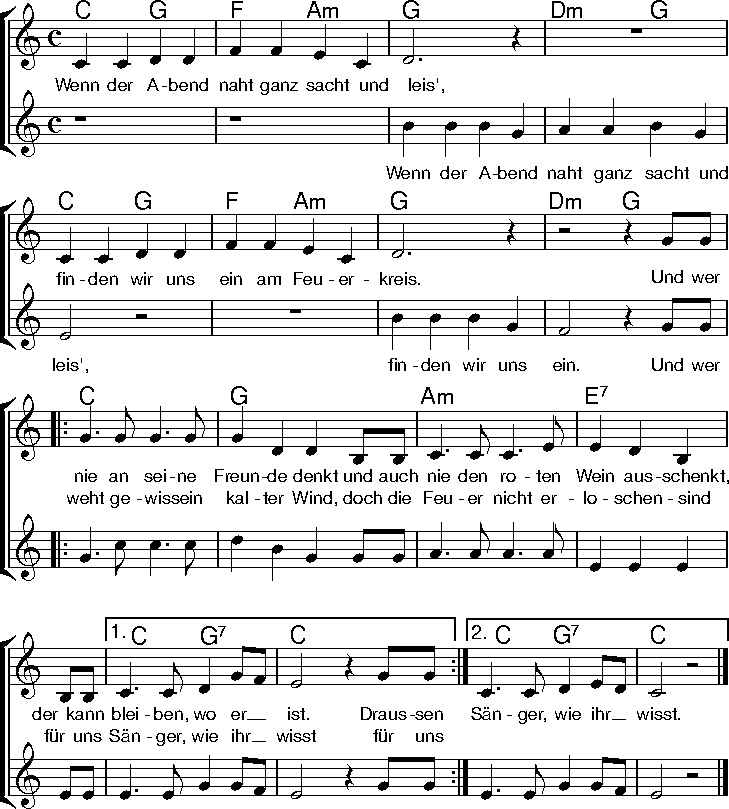
\includegraphics[width=1\textwidth]{Noten/Lied095.pdf}

\beginverse
\[C]Schatten \[G]flackern \[F]am Ru\[Am]inen\[G]rand, \[Dm] \[G]
\[C]hat das \[G]Singen \[F]dich nicht \[Am]längst ge\[G]bannt? \[Dm] \[G]
\endverse

\beginchorus
Und wer \[C]nie an seine \[G]Freunde denkt und auch \[Am]nie den roten \[E]Wein ausschenkt, 
der kann \[C]bleiben\[G7] wo er \[C]ist.
Draußen \[C]weht gewiss ein \[G]kalter Wind, doch die \[Am]Feuer nicht er\[E]loschen sind,
\lrep für uns \[C]Sänger, \[G7]wie ihr \[C]wisst. \rrep

\endchorus


\beginverse
^Wer da ^glaubt er ^könnt' all^eine ^geh'n, ^ ^
^wird in ^dieser ^Welt sehr ^leicht ver^weh'n. ^ ^
\endverse

\renewcommand{\everychorus}{\textnote{\bf Refrain (wdh.)}}
\beginchorus
\endchorus

\endsong

\begin{intersong}
\ifthenelse{\boolean{pics}}{
    \ThisLRCornerWallPaper{1}{Bilder/RV_WennDerAbendNaht.jpg}
}{}
\end{intersong}